%%%%%%%%%%%%%%%%%%%%%%%%%%%%%%%%%%%%%%%%%%%%%%%%%%%%%%%%%%%%%%%%%%%%%%%%%%%%
% AGUJournalTemplate.tex: this template file is for articles formatted with LaTeX
%
% This file includes commands and instructions
% given in the order necessary to produce a final output that will
% satisfy AGU requirements, including customized APA reference formatting.
%
% You may copy this file and give it your
% article name, and enter your text.
%
%
% Step 1: Set the \documentclass
%
% There are two options for article format:
%
% PLEASE USE THE DRAFT OPTION TO SUBMIT YOUR PAPERS.
% The draft option produces double spaced output.
%

%% To submit your paper:
\documentclass[draft]{agujournal2019}
\usepackage{url} %this package should fix any errors with URLs in refs.
\usepackage{lineno}
\usepackage{color}
\graphicspath{ {figures/} }
\linenumbers
%%%%%%%
% As of 2018 we recommend use of the TrackChanges package to mark revisions.
% The trackchanges package adds five new LaTeX commands:
%
%  \note[editor]{The note}
%  \annote[editor]{Text to annotate}{The note}
%  \add[editor]{Text to add}
%  \remove[editor]{Text to remove}
%  \change[editor]{Text to remove}{Text to add}
%
% complete documentation is here: http://trackchanges.sourceforge.net/
%%%%%%%

\draftfalse

\journalname{JGR: Space Physics}


\begin{document}

\title{Statistical Properties of Curtain Electron Precipitation Derived with AeroCube-6}

%% ------------------------------------------------------------------------ %%
%
%  AUTHORS AND AFFILIATIONS
%
%% ------------------------------------------------------------------------ %%

\authors{M. Shumko\affil{1}, A.T. Johnson\affil{1}, J.G. Sample\affil{1}, D.L. Turner\affil{3}, T.P. O'Brien\affil{2}, and J.B. Blake\affil{2}}


\affiliation{1}{Department of Physics, Montana State University, Bozeman, Montana, USA}
\affiliation{2}{Space Science Applications Laboratory, The Aerospace Corportation, El Segundo, California USA}
\affiliation{3}{Johns Hopkins Applied Physics Laboratory, Laurel, Maryland, USA}

\correspondingauthor{M. Shumko}{msshumko@gmail.com}

\begin{keypoints}
\item We used the dual AeroCube-6 CubeSats to identify stationary, narrow, and persistent $>30$ keV precipitation in low Earth orbit
\item A single low Earth-orbiting spacecraft can easily misidentify curtains as microburst precipitation
\item A few curtains were persistently scattered into the atmosphere for at least six seconds
\end{keypoints}


\begin{abstract}
Abstract here
\end{abstract}

\section{Plain Language Summary}

\section{Introduction}
\textcolor{blue}{
Outline
\begin{enumerate}
\item Introduce various particle loss mechanisms
\item Introduce microbursts and their effect on atmospheric chemistry. Maybe mention how there is an unexplained source of HOX and NOX?
\item Introduce curtains and the prevailing hypothesis linking curtains to microbursts
\item If curtains are drifting then we have overestimated the atmospheric losses due to microbursts 
\item Our goal is to study three statistical properties of curtains: location, spatial width, and preferred geomagnetic conditions. Lastly we will use the SAA to determine if some curtains were drifting around the Earth or locally and persistently precipitating
\item Explain DLC and BLC. DLC description from Comes 2003 paper and maybe something from Craig Rogers group.
\item Maybe cite the curtain paper from 2000 that relates them to lightning? Title: Trapped energetic electron curtains produced by thunderstorm driven relativistic runaway electrons
\end{enumerate}
}

\textcolor{red}{Double check that I am citing correct references}
One of the important loss mechanisms of radiation belt electrons and protons is wave-particle scattering. A few wave modes have been extensively studied to scatter waves, EMIC, hiss, and chorus waves. EMIC wave excitation is believed to be caused by anisotopic distributions of $\approx 10$ keV protons injected from the magnetotail; while chorus waves are excited by $\approx 10$ keV electrons. Once excited, these waves scatter inner magnetosphere particles into the atmosphere. One form of precipitation that is widely believed to be caused by scattering between chorus waves and electrons in the outer radiation belts is microbursts. Microbursts are a spiky increase of electrons observed for shorter than a second. They have been studied since the mid 1960s with high altitude balloons and satellites \cite<e.g.>{Anderson1964, Lorentzen2001a, O'Brien2003, Douma2017}. The microburst impact on the environment has been estimated to be substantial. \citeA{Douma2019} and \citeA{Breneman2017} shown that microbursts can deplete the outer radiation belt electrons in around a day. Furthermore, \citeA{Seppala2018} modeled a 6 hour microburst storm and concluded that microbursts depleted mesospheric ozone by roughly 10\%.

With one spacecraft in low Earth orbit (LEO), moving at a typical 7.5 km/s velocity, it is impossible to differentiate between a microburst that gets scattered and lost in less than a second (temporal), and a stationary spiky feature that is narrower than 7 kilometers. Two identically-instrumented spacecraft orbiting in proximity can successfully differentiate between the two realities. One such mission is the dual AeroSube-6 (AC6) CubeSats that measured electrons and protons together in LEO between 2014 and 2017. With AC6 both structures were readily observed and studied: microbursts in \citeA{Shumko2020}, and recently discovered stationary, narrow, and spiky precipitation features called curtains that were first reported by \citeA{Blake2016}.

\subsection{Curtain Hypothesis}
Besides a brief description of curtains in \citeA{Blake2016}, not much is known about about them. \citeA{Blake2016} proposed an outstanding hypothesis that curtains are remnants of microbrusts that are not completely scattered into the atmosphere and over time the packet of microburst electrons is smeared out (bounce phase averaged) along the magnetic field line between the two hemispheres. Since different energy electrons drift around the Earth at different speeds, the electrons are not only smeared out along one field line, but also stretched out along the electron drift orbit into a curtain shape. In most regions in LEO where AC6 observes curtain electrons, these electrons are drifting east in the drift loss cone until they are scattered in the atmosphere in the South Atlantic Anomaly (SAA). The SAA is a region where Earth's magnetic field is weakest near the surface, caused by the spatial offset of Earth's magnetic field. A related region, magnetically conjugate to the SAA is the bounce loss cone (BLC). Traditionally, the BLC is defined as the North Atlantic region where if an electron is observed in LEO, it will either precipitate in the atmosphere below the spacecraft, or mirror at the spacecraft altitude and then potentially mirror at or below 100 km altitude in the SAA. At sub-100 kilometer altitude, collisions with the atmosphere are numerous and the particle will be lost. In this study we will assume this definition and a more strict definition that the particle will mirror at or below sea level in the SAA---in other words the particle is surely lost.

The concept of the bounce loss cone (BLC) pitch angle is traditionally defined as the pitch angle of a particle that will mirror at or below 100 km where collisions with the atmosphere become more numerous and the particle is likely to be lost within one bounce period. The BLC pitch angle, however small, is always defined but most LEO spacecraft do not have the angular resolution to identify particles that will be immediately lost. A particle can also be pseudo-trapped if it has a pitch angle between the BLC and the drift loss cone. A particle with a pitch angle smaller than the drift loss cone and larger than the BLC will locally mirror above 100 km and drift around the Earth until the altitude of the mirror point magnetic field descends below 100 km in the SAA and the particle is lost. For pitch angles greater than the drift loss cone, the particle is considered trapped.

Without the angular resolution necessary to study the particles in the BLC and DLC, the geographic location of the LEO spacecraft can be used to partially differentiate between the different populations. For most locations outside of the SAA, a LEO statecraft does not observe trapped particles and thus observes particles in the DLC and BLC. Those particles must be lost soon but the question remains if the particles are lost immediately or when they drift into the SAA. The region magnetically conjugate to the SAA in the north Atlantic ocean in also confusingly called the BLC. In the BLC region a particle either precipitates below the satellite, or mirror just below the satellite and precipitate in the SAA, where the particle’s mirror point in the SAA’s reduced magnetic field strength is lower in the atmosphere. In other words, the electron will be lost to the atmosphere. Thus in the BLC region any observed particle is lost within a bounce period (≈ 1 second for 30 keV electrons). Since AC6 does not have angular resolution, BLC will only refer to the north Atlantic region.

\textcolor{red}{OLD: I propose to test this question using Earth’s asymmetric magnetic field which creates a region of weaker magnetic field in the South Atlantic Anomaly (SAA). A related region, magnetically conjugate to the SAA in the North Atlantic, is the bounce loss cone (BLC). The BLC and the SAA are critical to test the proposed science question. A particle observed in LEO and in the BLC will precipitate within one bounce period (≈ 1 second for 35 keV electrons). The electron will either precipitate below the satellite, or mirror just below the satellite and travel into the SAA, where the particle’s mirror point in the SAA’s reduced magnetic field strength is deep in the atmosphere. In other words, the electron will transfer its energy and be lost to the atmosphere.}


\section{Instrumentation} \label{instrumentation}
\textcolor{blue}{Think about the flow, and avoid plagiarizing myself}

The AC6 mission was a pair of 0.5U (10x10x5 cm) CubeSats built by The Aerospace Corporation designed to measure the electron and proton environment in low Earth orbit \cite{O'brien2016}. AC6 was launched on 19 June 2014 into a 620x700 km, $98^\circ$ inclination orbit. The AC6 orbit over the three year mission lifetime was roughly dawn-dusk, and precessed only a few hours in MLT; 8-12 MLT in dawn and 20-24 MLT in dusk. The two AC6 spacecraft, designated as AC6-A and AC6-B, separated after launch and were in proximity for the duration of the three year mission---maintained by an active attitude control system. The attitude control system allowed then to precisely control the amount of atmospheric drag experienced by each AC6 unit using the surface area of their solar panel ``wings". By changing their orientation, AC6 was able to maintain a separation between 2-800 km, confirmed with the Global Positioning System. The two AC6 units were in a string of pearls configuration so one unit, typically unit A, was leading the other by an in-track lag---the time it would take the following spacecraft to catch up to the position of the leading spacecraft. To convert between the AC6 in-track separation and in-track lag, we assume a typical 7.5 km/s orbital velocity of LEO spacecraft. The in-track lag was readily available with the Global Positioning System which makes it easy to study precipitation phenomena observed at the same time, and at the same position by shifting one time series by the in-track lag.

Each AC6 unit contains three Aerospace microdosimeters (licensed to Teledyne Microelectronics, Inc) that measure the electron and proton dose in orbit \cite{O'brien2016}. The dosimeter used for this study is dos1 with a $30$ keV electron threshold. dos1 is used for this study because the other dosimeters were not identical between unit A and B. All dosimeters sample at 1 Hz in survey mode, and 10 Hz in burst mode. 10 Hz data was readily available from both AC6 units from June 2014 to May 2017 while their in-track lag was less than 65 seconds, and at times was a fraction of a second. \textcolor{red}{Show a distribution of the in-track lag when they had 10 Hz data?} The variety of AC6 separations and data availability over the three-year mission makes it possible to study tranisent electron microburst precipitation \cite{Shumko2020} and now stationary electron curtain precipitation.

\iffalse
The AC6 mission consists of a pair of 0.5U (10x10x5 cm) CubeSats built by The Aerospace Corporation and launched on June 19th, 2014 into a 620 x 700 km, $98^\circ$ inclination orbit. The two satellites, designated as AC6-A and AC6-B, separated after launch and drifted apart. Both AC6 units have an active attitude control system which allows them to adjust the atmospheric drag experienced by each AC6 unit by orienting their solar panel ``wings" with respect to the ram direction. By changing their orientation, the AC6 mission was able to achieve fine separation control and maintain a separation between 2-800 km, which was confirmed with GPS. Figure \ref{fig1}a shows the AC6 separation for the duration of the mission. Figure \ref{fig1}b shows where both AC6 units were taking 10 Hz data simultaneously as a function of L and MLT which highlights that most data were taken at 8-12 MLT, an ideal local time for observing microbursts. Lastly Fig. \ref{fig1}b shows that over a three year period the AC6 orbit was roughly dawn-dusk, sun-synchronous, and precessed 8 to 12 MLT in the dawn region. AC6's 8-12 MLT precession is ideal for sampling the region where microbursts are most likely to be observed \cite<e.g.>{O'Brien2003} but the tradeoff is limited microburst size information in MLT.

Each AC6 unit is equipped with three Aerospace microdosimeters (licensed to Teledyne Microelectronics, Inc). The dosimeter used for this study, dos1, is identical on both AC6 units and has a $35$ keV electron threshold. All AC6 dosimeters sample at 1 Hz in survey mode, and 10 Hz in burst mode in the radiation belts  \cite{O'brien2016}. Since microburst duration is less than a second, only the 10 Hz data was used to identify microbursts. \fi

\section{Methodology} 
\subsection{Curtain Identification} \label{curtain_identification}
\textcolor{blue}{
Outline
\begin{enumerate}
\item Various parameters were explored and we tuned it to have as many candidate events as possible while being feasible to inspect every detection. 
\item Baseline sensitivity decreases with larger structures, depending on the curtain amplitude, background level, and baseline width. Sensitivity begins to rapidly diminish for widths close to half of the baseline width---around five seconds, correspondent to 38 km size, for this identification criteria.
\end{enumerate}
}

The 10 Hz data was used to identify curtains with the following two criteria: a high spatial correlation, and \textcolor{red}{bursty}. The first criterion quantifies the similarity of the feature between both AC6 units, and the second criterion checks that highly correlated times were \textcolor{red}{bursty}. Before we we applied the identification criteria, the AC6-B time series was shifted by the in-track lag to spatially align it with the AC6-A time series. 

The first identification criterion is a 1-second rolling Pearson correlation applied to both time series. Spatial features with a correlation greater than 0.8 were considered highly correlated and saved.

The second identification criterion checks for locations where both AC6 units observed \textcolor{red}{bursty} precipitation. Similar to how precipitation bands were identified in \citeA{Blum2015} and microbursts in \citeA{Greeley2019}, we find \textcolor{red}{bursty} precipitation by estimating the number of Poisson standard deviations, $\sigma$, that a dos1 count rate is above a centered 10-second running average, $B_{10}$. Locations where the count rates are at least two $\sigma$ above $B_{10}$ are bursty. 

The locations where the two criteria are met are curtain candidates and the time of the peak count rates are saved. To check the quality of the data set, one author visually checked every candidate curtain and 1634 curtains were confirmed. Four curtain examples are shown in Fig. \ref{fig1}. In these examples the unmodified time series is in the top row and the corresponding spatially-aligned time series is in the bottom row. The in-track lag used to shift the bottom row is annotated by $dt$, corresponding to an AC6 in-track separation annotated by $s$. The top row is uncorrelated; thus these events were not microbursts. The bottom row is correlated after 3 to 26 seconds. The correlated curtains in the bottom row are peculiar---they have a fine structure on a 10-kilometer scale that we have shown to persist for at least 26 seconds.

%on fine time scales as short as a second

\begin{figure}
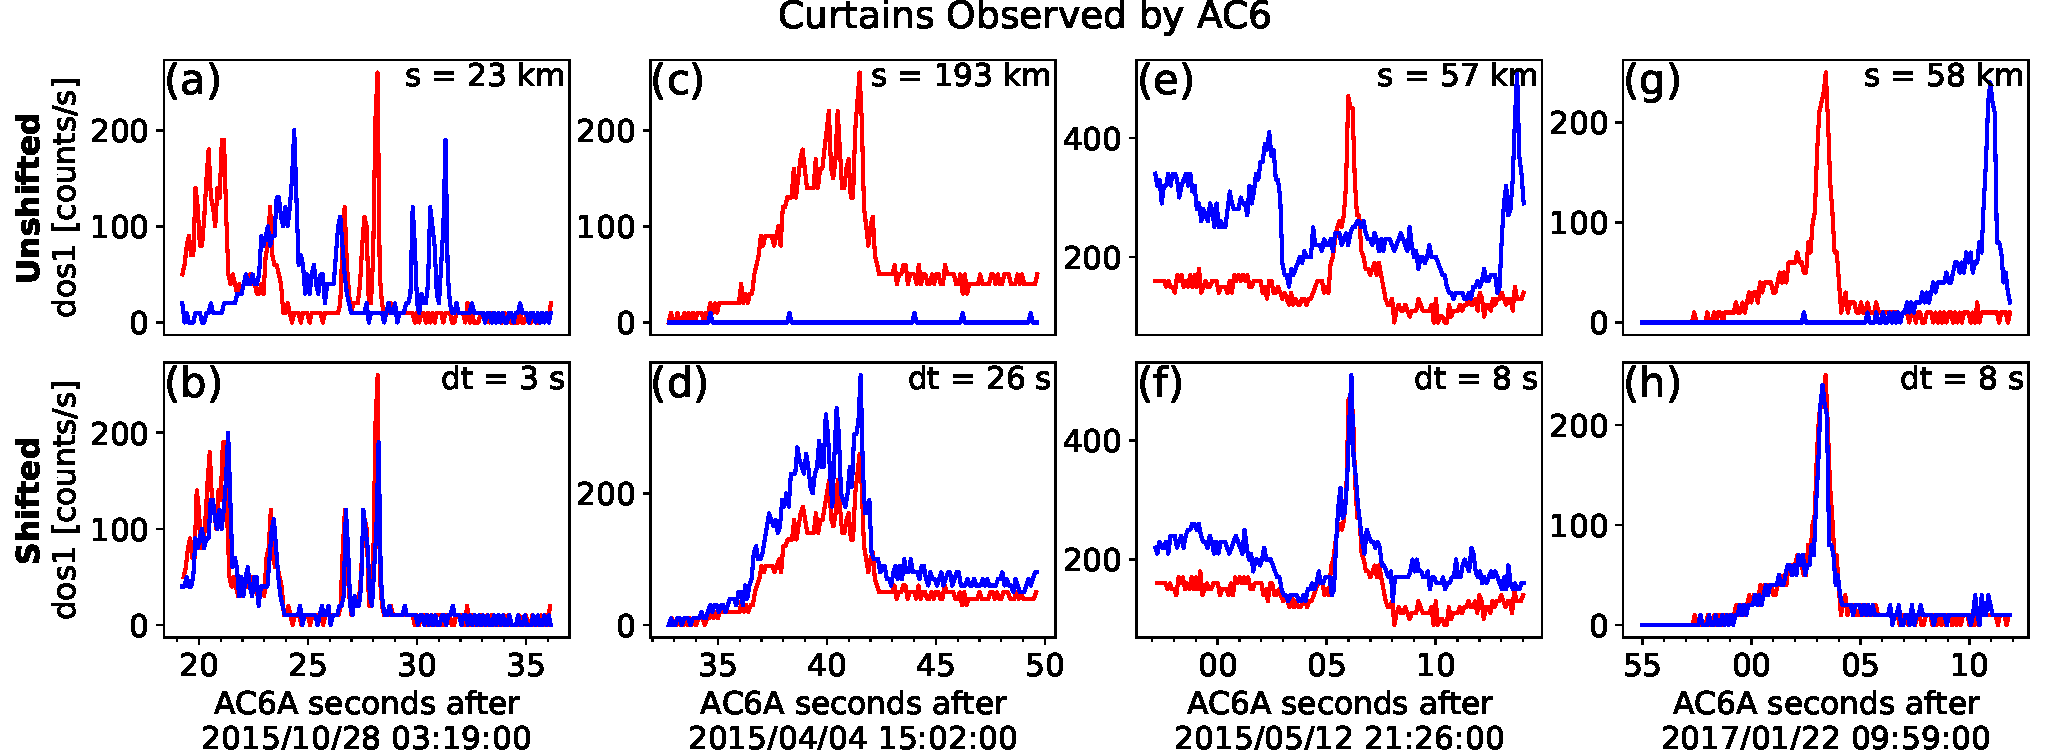
\includegraphics[width=\textwidth]{fig1.pdf}
\caption{Four examples showing the AC6 $> 30$ keV electron data taken by AC6 at the same time in the top row and at the same position in the bottom row. AC6-A, whose data is shown with red curves, was $s$ kilometers ahead of AC6-B. To show the data at the same position the time series data from one spacecraft was shifted by the in-track lag and annotated by dt. These examples show curtain precipitation that was highly correlated for up to 26 seconds.}
\label{fig1}
\end{figure}

\section{Results} \label{results}
\textcolor{blue}{
Outline
\begin{enumerate}
\item Show curtain width and comment how narrow they are. Whether they are drifting or locally precipitating, they must have a very filamentary structure that persists for multiple seconds
\item Figure out how the detection bias affects the width distribution
\item Show, and comment on the Auroral electroject strengths when each curtain was observed. Curtains are more likeliy to be observed during disturbed times.
\item Discuss the SAA, BLC, and show the curtains the the BLC plot. Mention how these electrons must have been precipitating for multiple seconds, over an order of magnitude longer than typical microbursts.
\end{enumerate}
}

In the spirit of brevity, we limited the scope of this statistical study to answer three questions:

\begin{enumerate}
\item how narrow are curtains,
\item when and where are curtains observed, and
\item are curtains drifting or locally precipitating?
\end{enumerate} For each of these questions we will compare the curtain distribution against the $>30$ keV microburst distribution from \citeA{Shumko2020}. Then we will provide observational evidence that suggests that some curtain electrons are continuously scattered and can not be drifting.

\subsection{Statistical Properties}
We quantified curtain width in time as the width at half of the curtain's topographic prominence: the height of the peak above the lowest contour that encircles the peak but contains no higher peak. The spatial width along the in-track direction, mostly in latitude. The distribution of curtain widths is shown in Fig. \ref{ae_width_dist} by the thick black curve. 

\begin{figure}
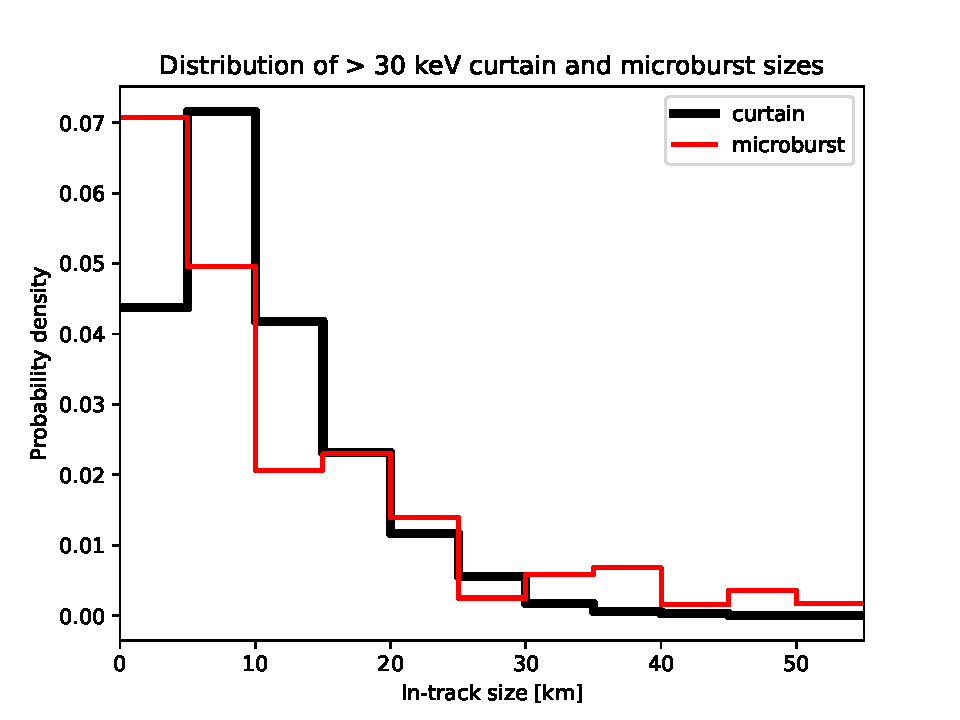
\includegraphics[width=\textwidth]{ac6_curtain_microburst_width_dist.pdf}
\caption{Size distributions of curtains (AC6 in-track separation mostly in latitude) in black and microbursts in red as a function of AC6 in-track width. Microburst distribution adopted from \citeA{Shumko2020}.}
\label{ae_width_dist}
\end{figure}

\begin{figure}
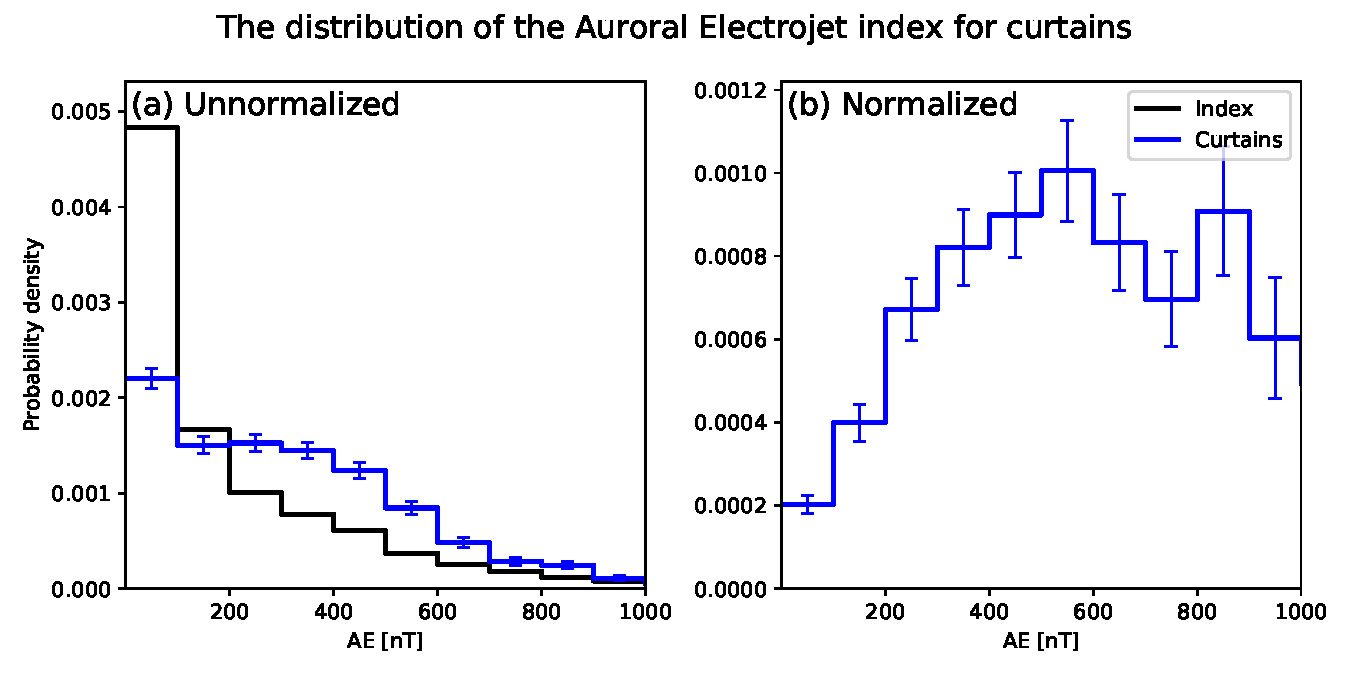
\includegraphics[width=\textwidth]{ac6_curtain_AE_dist.pdf}
\caption{The distribution of the Auroral Electroject index from 2014 to 2017 shown by the thick black curve, and the Auroral Electroject index when curtains were observed by the red curve.}
\label{ae_width_dist}
\end{figure}

\begin{figure}
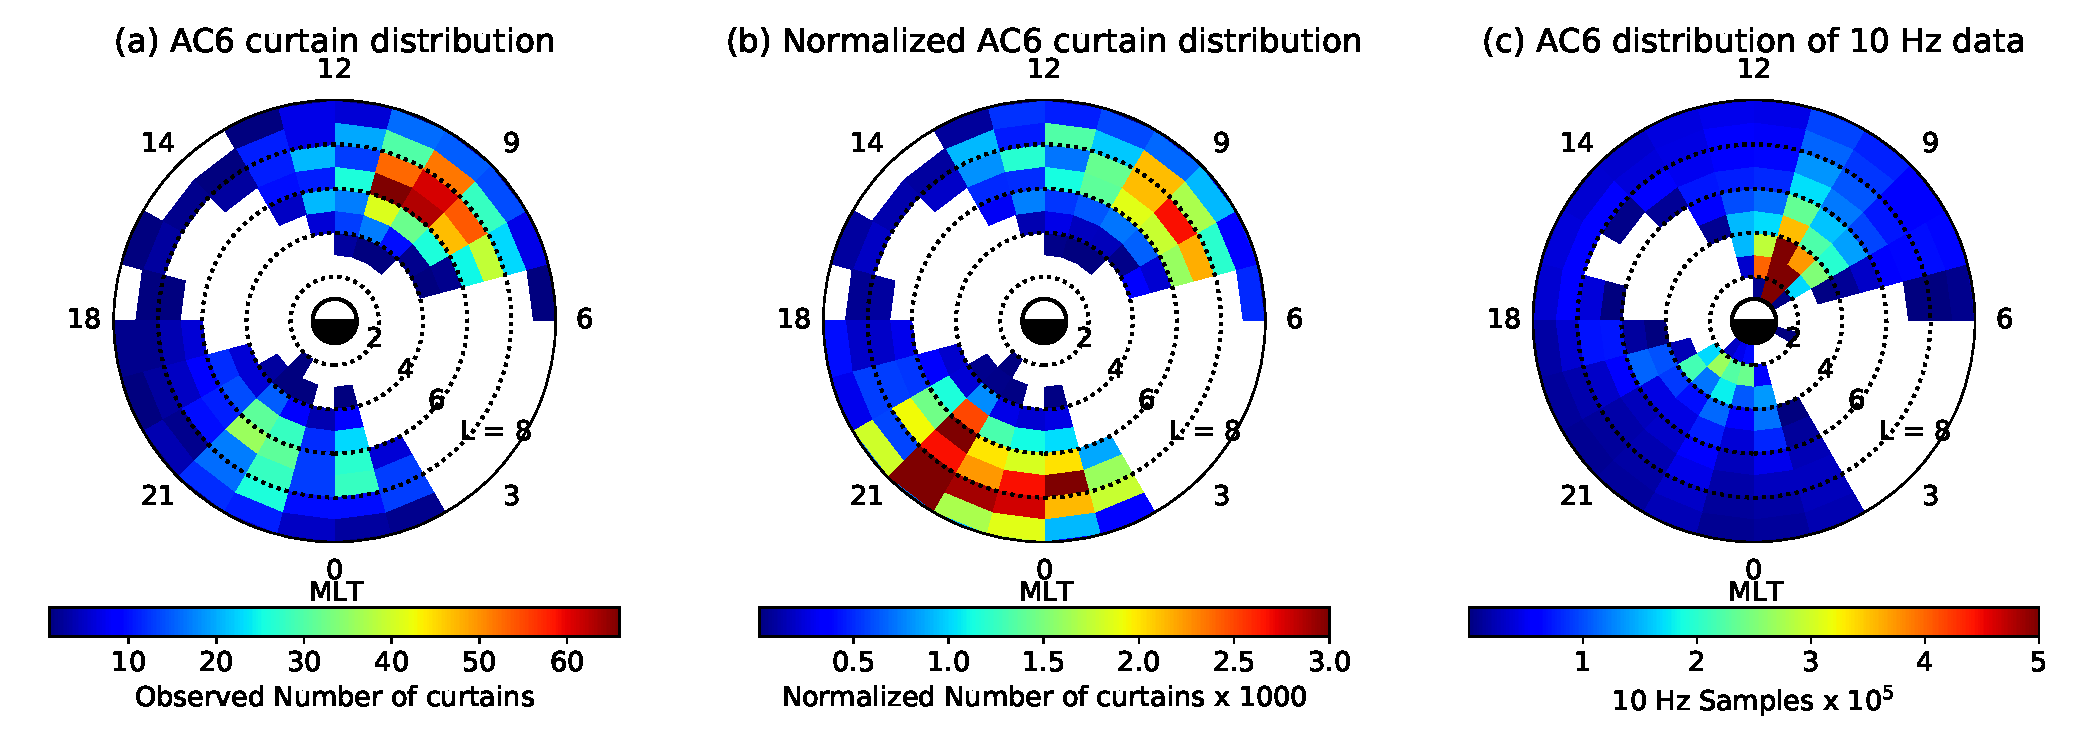
\includegraphics[width=\textwidth]{fig2_2.pdf}
\caption{Distribution of curtains as a function of L and MLT. White bins have 0 curtain detections or 10 Hz samples. Furthermore, to avoid noisy normalization scaling in panel b, bins with less than $10,000$ 10 Hz samples are shaded white.}
\end{figure}

\begin{figure}
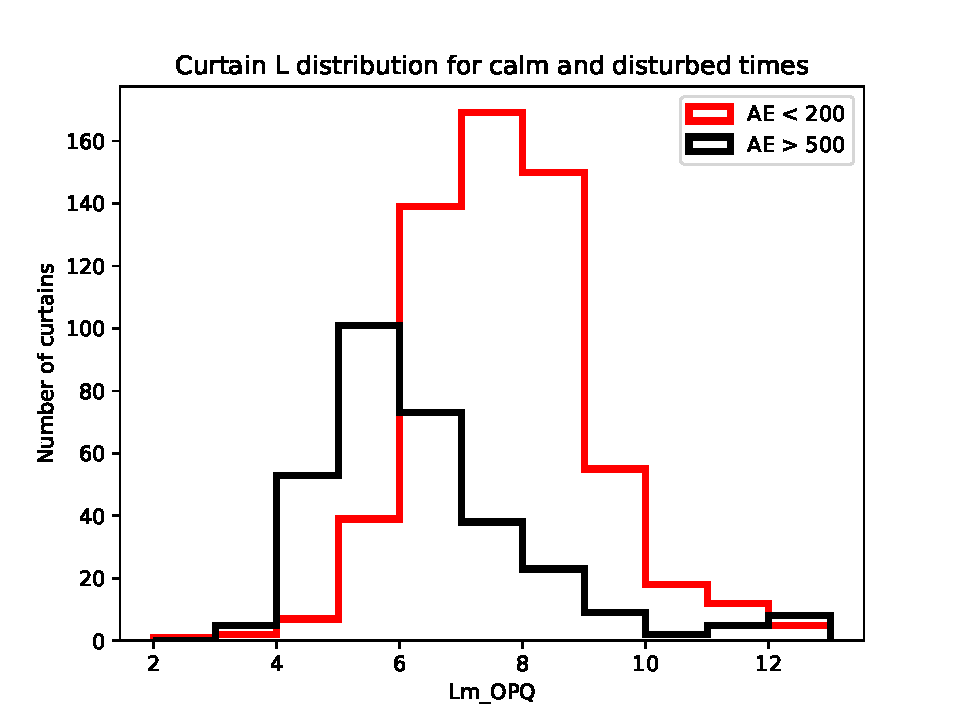
\includegraphics[width=\textwidth]{curtain_L_vs_AE.pdf}
\caption{\textcolor{red}{What about this figure?}}
\end{figure}

\subsection{Local Atmospheric Precipitation}
\begin{figure}
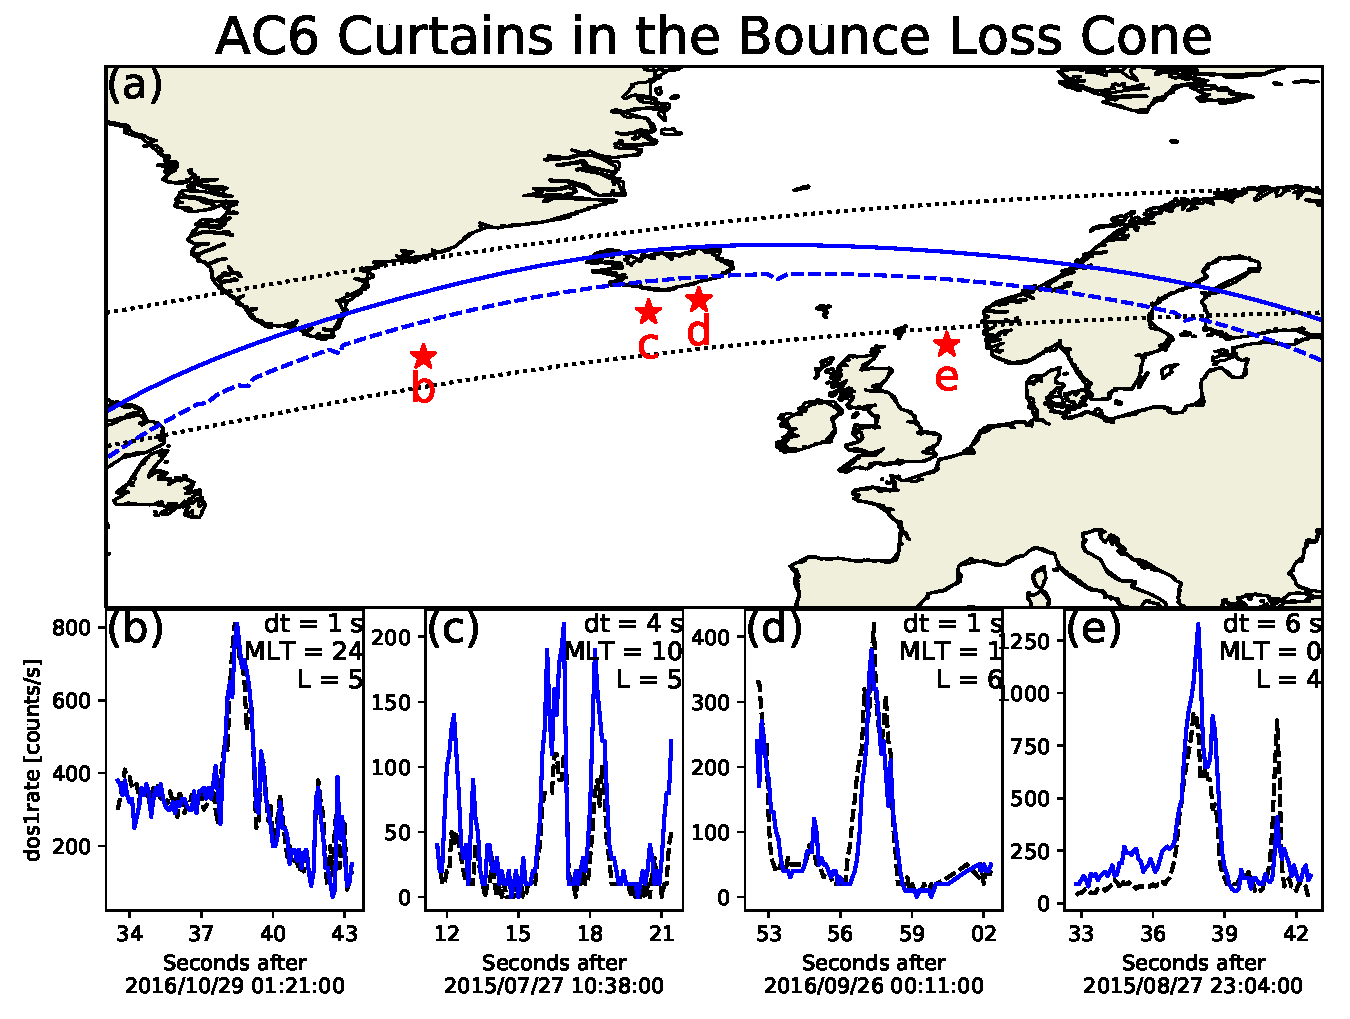
\includegraphics[width=\textwidth]{fig3.pdf}
\caption{Curtains observed inside the bounce loss cone. \textcolor{red}{Refrence Comess 2013 and DIETRICH 2010 paper that shows a similar BLC region.}}
\label{fig3}
\end{figure}

\section{Discussion} \label{discussion}
\textcolor{blue}{
Outline
\begin{enumerate}
\item Curtains are spatially small and must be around a few hundred km at the equator
\item curtain phenomena originates in the outer radiation belt, and observed relatively more in the evening than morning regions. Limited AC6 coverage prevents a complete MLT distribution
\item preference to disturbed conditions
\item some curtains locally precipitate for an extended period of time so there must be a sustained parallel electric field. Show the derivation and estimated potential.
\item AC6 can't answer this question, but curtains could provide a substantial source of HOx and NOX molecules responsible for destroying ozone. We need AC6 with energy and pitch angle resolution.
\end{enumerate}}

\section{Conclusions}

% \appendix

\acknowledgments
This work was made possible with the help from the many engineers and scientists at The Aerospace Corporation who designed, built, and operated AC6. M. Shumko was supported by NASA Headquarters under the NASA Earth and Space Science Fellowship Program - Grant 80NSSC18K1204. D.L. Turner is thankful for support from the Van Allen Probes mission and a NASA grant (Prime award number: 80NSSC19K0280). The work at The Aerospace Corporation was supported in part by RBSP-ECT funding provided by JHU/APL contract 967399 under NASA's Prime contract NAS501072. The AC6 data is available at http://rbspgway.jhuapl.edu/ac6 and the IRBEM-Lib version used for this analysis can be downloaded from https://sourceforge.net/p/irbem/code/616/tree/.

\section{Homeless Words}

Title: Statistical Properties of Curtains--Latitudinally-Narrow and Persistent Electron Precipitation Phenomena

This study leverages AC6, a multi-spacecraft mission, to interpret and understand particle precipitation in a way that is impossible with a single spacecraft.

This study leverages the asymmetry in Earth's magnetic field. The asymmetric magnetic field results in the SAA and the BLC, two very related and unique regions

Particles that impact the atmosphere are lost during that bounce motion. We found curtains in the bounce loss cone, a region in the North Atlantic near and above Iceland.

The bounce loss cone is magnetically connected to the SAA, where Earth's magnetic field is weakest near Earth's surface. A particle observed in the blc in the northern hemisphere will descend below 100 km altitude. At sub-100 km altitudes the particle has a high chance of encountering and scattering with the atmosphere and be lost. 

We found curtain electrons that, when given the chance to execute their cyclical bounce motion, will descend below Earth's surface in the SAA. An electrons can not survive that trip.

Write the paper and ask the question: "What is this paper really about?" Not just curtains, but uncovering something unexpected that has been observed and overlooked for decades.

Are curtains related to aurora? This is a good question---one that is not pertinent here (idea from The Elements of Style p.68).

Here are two parting questions that are not considered here. Why were some curtains shifted slightly? Perhaps it was due to the movement of the magnetic field lines. Also do curtains have a corresponding visual signature on the ground? The answer to this question will show if curtains are related to the aurora.

\bibliography{/home/mike/Dropbox/0_firebird_research/A_presentations/refs}
%\bibliography{"refs"}

\end{document}